\documentclass[preprint,12pt]{elsarticle}
\usepackage{lineno}
\usepackage{tikz}

\journal{WebPhysics}

\begin{document}
\begin{frontmatter}
\title{Parallel Physics Engine for the Front End}
\author{Kai Matsuda (Vangogh500)}
\address{MA, US}
\begin{abstract}
Physics simulations on the web has always sacrificed convenience for performance due to the limitations of the browser. With the introduction of web workers and the ability for content to run on multiple threads, this tradeoff can be further minimized. Utilization of this new technology could help bring physics simulations to the web in order to benefit from the web's ease of access and usability.
\end{abstract}
\end{frontmatter}
\linenumbers
\section{Hierarchy}
A world ($W$) represents a system of rules that is being observed. An environment ($E$) represents an observed rule or a law of physic. A body ($B$) represents a single entity of interest that is being observed. A component ($C$) is a characteristic of a particular body that may be of interest i.g. position or rotation. Each world ($W_i$) has a set of environments ($S_i^E$) that are part of the simulation. Each environment ($E_i$) has a set of bodies ($S_i^B$) that must conform by its rule, and each body ($B_i$) has a set of components ($S_i^C$).
\[ S_i^E = \{ E_1, E_2, E_3... \} \]
\[ S_i^B = \{ B_1, B_2, B_3... \} \]
\[ S_i^C = \{ C_1, C_2, C_3... \} \]
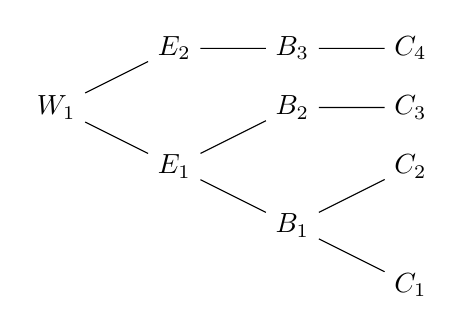
\begin{tikzpicture}[
	grow = right
]
\node{$W_1$}
	child{node{$E_1$}
		child{node{$B_1$}
			child{node{$C_1$}}
			child{node{$C_2$}}
		}
		child{node{$B_2$}
			child{node{$C_3$}}
		}
	}
	child{node{$E_2$}
		child{node{$B_3$}
			child{node{$C_4$}}
		}
	};
 
\end{tikzpicture}
\section{Components}
A component $C$ is represented as a parametric function $C(t)$ with time input $t$. Components should be able to be constructed using the raw parametric equation or by specifying n-levels of derivatives. Let $C^*$ represent the constructor.
\[C^*(<0,-1/2,0>gt^2+<2,0,0>t)= C(t) = <0,-1/2,0>gt^2+<2,0,0>t \]
\[C^*(<0,0,0>,<2,0,0>,<0,-1/2,0>)= C(t) = <0,-1/2,0>gt^2+<2,0,0>t \]

Each component can thus be concurrently calculated. Let $C_i^t$ be identified where t represents $C_i(t)$

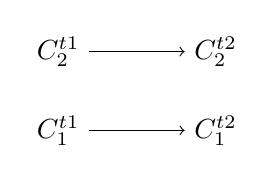
\begin{tikzpicture}[
	grow = right
]
\node (A1) at (0,0) {$C_1^{t1}$};
\node (A2) at (2,0) {$C_1^{t2}$};
\node (B1) at (0,1) {$C_2^{t1}$};
\node (B2) at (2,1) {$C_2^{t2}$};

\draw[->]
	(A1) edge (A2) (B1) edge (B2);
\end{tikzpicture}

\section{Bodies}


\end{document}